% !TeX root = thesis.tex
%--------------------------------------------------------------------%
%
% Template TA LaTeX Teknik Informatika ITERA.
% Editor: Radhinka Bagaskara, Martin C.T. Manullang, iwawiwi
% Version 2024.1
%
% Berdasarkan "Templat LaTeX Tesis Informatika ITB" oleh Petra Barus & Peb Ruswono Aryan
% https://github.com/petrabarus/if-itb-latex
%--------------------------------------------------------------------%
%
% Berkas ini berisi struktur utama dokumen LaTeX yang akan dibuat.
%
%--------------------------------------------------------------------%

% Set jenis dokumen Tugas Akhir
\documentclass[12pt, a4paper, onecolumn, oneside, final]{report}
% \documentclass[11pt, a5paper, onecolumn, final]{report} % Untuk versi perpustakaan

%-------------------------------------------------------------------%
%
% Konfigurasi dokumen LaTeX untuk laporan tesis IF ITB
% 
%
% @author Radhinka Bagaskara, Petra Novandi (ITB)
%
%-------------------------------------------------------------------%
%
% Berkas asli berasal dari Steven Lolong
%
%-------------------------------------------------------------------%

% Import package penting
\usepackage[utf8]{inputenc}
\usepackage{subcaption} % Paket untuk mengatur gambar berdampingan
\usepackage{graphicx}
\usepackage{titling}
\usepackage{blindtext} % Untuk lorem ipsum
\usepackage{sectsty} % Untuk header & judul
\usepackage{chngcntr} % Untuk penambahan nomor caption
\usepackage{etoolbox} % Untuk CRUD variabel (?)
\usepackage{array} % % Untuk tabel di math mode
\usepackage{float} % Untuk tabular
\usepackage{longtable} % Untuk tabel yang potong halaman
\usepackage{amsmath} % Untuk equation
\usepackage{enumitem} % Untuk list enumerate yg lebih rapi
\usepackage[bookmarks]{hyperref}
\hypersetup{
	colorlinks,
	citecolor=black,
	filecolor=black,
	linkcolor=black,
	urlcolor=black
}

% Ukuran kertas A4
\special{papersize=210mm,297mm}

% Setting margin
\usepackage[top=3cm,bottom=3cm,left=3.5cm,right=3cm]{geometry}

% Setting indensasi
\usepackage{indentfirst}
\usepackage{parskip}
\setlength{\parindent}{20pt}
\setlength{\parskip}{10pt}

% Linespacing 1.5. Tidak serupa dengan 1.5 di Word (RDB)
\renewcommand{\baselinestretch}{1.5}

% Agar tidak ada kata yang terpotong setiap baris kalimat
\hyphenpenalty=10000

% Font
%\usepackage{mathptmx} 
\usepackage{newtx} 
% Times New Roman itu copyright dari Microsoft. Ini alternatifnya (RDB)

% Judul bahasa Indonesia
\usepackage[bahasa]{babel}

% Format tanggal
\usepackage[style=ddmmyyyy,datesep=-]{datetime2}



% Format citation
\usepackage[backend=biber,citestyle=ieee]{biblatex}

% Remove "In:" before journal titles
\renewbibmacro{in:}{}

% Ensure URLs, DOIs, and ISSNs use the default font (e.g., Times New Roman)
\renewcommand*{\UrlFont}{\rmfamily} % Use default font for URLs
\DeclareFieldFormat{issn}{#1}       % Use default font for ISSN
\DeclareFieldFormat{doi}{#1}        % Use default font for DOI

% Remove DOI and URL fields if not needed (optional)
\AtEveryBibitem{
  \clearfield{doi}
  \clearfield{url}
}

\DeclareLanguageMapping{bahasa}{english}



% Package untuk link di daftar isi.
\usepackage{titlesec}       % Package Format judul
\usepackage{parskip}
\usepackage{ragged2e}		% Alignment
\usepackage{multirow}		% Untuk bisa merge cell di tabel
\usepackage{tikz}			% Untuk menggambar kotak pas foto
\usepackage{setspace}		% Spacing paragraph
\usepackage{fancyhdr}		% Agar nomor halaman di pojok kanan atas
\usepackage{caption} 		% Caption gambar & tabel

% Setting supaya nomor halaman pertama dengan "chapter"
% berada di kanan atas
\fancypagestyle{plain}{%
	\fancyhf{}%
	\renewcommand{\headrulewidth}{0pt}
	\fancyhead[R]{\thepage}
}

% Setting judul
\chapterfont{\centering \large}
\titleformat{\chapter}[display]%
  	{\large\centering\bfseries}%
  	{\chaptertitlename\ \thechapter}{0pt}%
  	{\large\bfseries\uppercase}
\titleformat{\section}%
	{\normalfont\normalsize\bfseries}{\thesection}{1em}{}
\titleformat{\subsection}%
	{\normalfont\normalsize\bfseries}{\thesubsection}{1em}{}
    
% Setting spacing di setiap judul chapter
\titlespacing*{\chapter}{0pt}{-30pt}{20pt}

% Setting nomor pada subbsubsubbab
\setcounter{secnumdepth}{3}

% Counter untuk figure dan table, agar bertambah walaupun lintas subbab
\counterwithout{figure}{section}
\counterwithout{table}{section}

% Supaya tidak ada garis di header
\renewcommand{\headrulewidth}{0pt}

% Setting daftar isi, daftar gambar, daftar tabel, daftar rumus
\usepackage[titles]{tocloft}
\setlength{\cftbeforechapskip}{5.2pt}
\cftsetindents{section}{1.5em}{2.3em}
\cftsetindents{subsection}{3em}{3em}
\setlength{\cfttabindent}{1.5em}
\setlength{\cftfigindent}{1.5em}

% Tambahkan kata "BAB" sebelum nomor bab di daftar isi
\renewcommand*\cftchappresnum{\MakeUppercase{BAB}~}
\renewcommand\chaptername{BAB}
\settowidth{\cftchapnumwidth}{\cftchappresnum}
\renewcommand{\cftchapaftersnumb}{\quad}
\addtocontents{toc}{
\protect\renewcommand*\protect\cftchappresnum{\MakeUppercase{\chaptername}~}
}

\renewcommand{\cftchapleader}{\dotfill} 
\renewcommand{\cftsecleader}{\dotfill}
\renewcommand{\cftsubsecleader}{\dotfill}
\renewcommand{\cftfigleader}{\dotfill}
\renewcommand{\cfttableader}{\dotfill}

% Nama daftar isi, gambar, tabel, rumus dalam bahasa Indonesia
\addto\captionsbahasa{%
	\renewcommand{\contentsname}{DAFTAR ISI}%
	\renewcommand{\listfigurename}{DAFTAR GAMBAR}%
	\renewcommand{\listtablename}{DAFTAR TABEL}%
}

% Setting daftar rumus
\newcommand{\listequationsname}{DAFTAR RUMUS}
\newlistof{myequations}{equ}{\listequationsname}
\newcommand{\myequations}[1]{
	\addcontentsline{equ}{myequations}{\protect\numberline{\theequation}#1}
}

% Mengatur format daftar rumus
\renewcommand{\cftmyequationspresnum}{Rumus\ }
\newlength{\mylenf}
\settowidth{\mylenf}{\cftmyequationspresnum}
\setlength{\cftmyequationsnumwidth}{\dimexpr\mylenf+1.5em} % Menyesuaikan nomor
\setlength{\cftmyequationsindent}{1.5em} % Menambahkan indentasi daftar rumus
\renewcommand{\cftmyequationsleader}{\dotfill}

% Setting daftar gambar dan daftar tabel
\renewcommand\cftfigpresnum{Gambar\ }
\renewcommand\cfttabpresnum{Tabel\ }
\settowidth{\mylenf}{\cftfigpresnum}
\setlength{\cftfignumwidth}{\dimexpr\mylenf+1.5em}
\setlength{\cfttabnumwidth}{\dimexpr\mylenf+0.5em}

% Setting penomoran caption gambar, tabel, dan rumus
\renewcommand{\thefigure}{\arabic{chapter}.\arabic{figure}}
\renewcommand{\thetable}{\arabic{chapter}.\arabic{table}}
\renewcommand\theequation{\arabic{section}.\arabic{equation}}

% Untuk mengganti nama bulan di babel bahasa
% tapi belum jalan (RDB)
\StartBabelCommands*{bahasa}{date}
\SetStringLoop{month#1name}{%
	Januari,Februari,Maret,April,Mei,Juni,%
	Juli,Agustus,September,Oktober,November,%
	Desember}
\EndBabelCommands     

% english title
\providecommand\titleEN[1]{\providecommand\thetitleEN{#1}}

% Saya lupa ini buat apa (RDB)
%\renewcommand{\theHsection}{\thepart.section.\thesection}

% Semua dibawah ini berhubungan dengan CRUD variabel (ada simbol @)
\makeatletter % Jangan dihapus

% Command untuk variabel NIM
\newcommand{\nim}[1]{\def\@nim{#1}}
\newcommand{\printnim}{\@nim}

% Command untuk variabel Dosen Pembimbing I & II
\newcommand{\namadosbinga}[1]{\def\@namadosbinga{#1}}
\newcommand{\namadosbingb}[1]{\def\@namadosbingb{#1}}
\newcommand{\nipdosbinga}[1]{\def\@nipdosbinga{#1}}
\newcommand{\nipdosbingb}[1]{\def\@nipdosbingb{#1}}
\newcommand{\printnamadosbinga}{\@namadosbinga}
\newcommand{\printnamadosbingb}{\@namadosbingb}
\newcommand{\printnipdosbinga}{\@nipdosbinga}
\newcommand{\printnipdosbingb}{\@nipdosbingb}
\newcommand{\dosbingA}[2]{\namadosbinga{#1} \nipdosbinga{#2}}
\newcommand{\dosbingB}[2]{\namadosbingb{#1} \nipdosbingb{#2}}

% Command untuk variabel Dosen Penguji I & II
\newcommand{\namapengujia}[1]{\def\@namapengujia{#1}}
\newcommand{\namapengujib}[1]{\def\@namapengujib{#1}}
\newcommand{\nippengujia}[1]{\def\@nippengujia{#1}}
\newcommand{\nippengujib}[1]{\def\@nippengujib{#1}}
\newcommand{\printnamapengujia}{\@namapengujia}
\newcommand{\printnamapengujib}{\@namapengujib}
\newcommand{\printnippengujia}{\@nippengujia}
\newcommand{\printnippengujib}{\@nippengujib}
\newcommand{\pengujiA}[2]{\namapengujia{#1} \nippengujia{#2}}
\newcommand{\pengujiB}[2]{\namapengujib{#1} \nippengujib{#2}}

% Command untuk merubah spacing equation
\g@addto@macro\normalsize{%
	\setlength\abovedisplayskip{-10pt}
	\setlength\belowdisplayskip{-10pt}
	\setlength\abovedisplayshortskip{-10pt}
	\setlength\belowdisplayshortskip{-10pt}
}

\makeatother % Jangan dihapus


% \input{config/config_perpus.sty} % Untuk versi perpustakaan

\bibliography{references}

\begin{document}
% 	\pagestyle{plain}
% 	\fancyhf{}
% 	\rfoot{Halaman \thepage}%

    %----------------------------------------------------------------%
    % Konfigurasi Informasi Tugas Akhir
    %----------------------------------------------------------------%
    
    % Judul Tugas Akhir
    \title{Analisis Algoritma ABC Untuk Pemecahan Masalah Penjadwalan Job Shop} % Judul Tugas Akhir dalam Bahasa Indonesia	
    % DITULIS DALAM HURUF KAPITAL; Font size 16 pt; Bold; Tidak melebihi 4 baris
    \titleEN{Comparison }      % Judul Tugas Akhir dalam Bahasa Inggris
    
    % Informasi Mahasiswa
    \author{Ardoni Yeriko Rifana Gultom}		% Nama Mahasiswa
	\nim{121140141}			% NIM Mahasiswa
	
	%Informasi Dosen Pembimbing
	\dosbingA%
		{Martin Clinton Tosima Manullang, Ph.D.}%	% Nama Dosen Pembimbing 1
		{NIP. 19930109 2019 03 1 017}				% NIP Dosen Pembimbing 1
	\dosbingB%
		{Nama dan Gelar Pembimbing II}%	% Nama Dosen Pembimbing 2
		{NIP. 123456789}				% NIP Dosen Pembimbing 2
		
	%Informasi Dosen Penguji
	\pengujiA%
		{Andika Setiawan, S.Kom., M.Cs.}%	% Nama Dosen Penguji 1
		{NIP. 19911127 2022 03 1 007}				% NIP Dosen Penguji 1
	\pengujiB%
		{Eko Dwi Nugroho, S.Kom., M.Cs.}%	% Nama Dosen Penguji 2
		{NIP. 19910209 2024 06 1 001}				% NIP Dosen Penguji 2

	\sloppy % mencegah text overflow. (Jose)
    \pagenumbering{roman}
    \setcounter{page}{1} % Nomor halaman dimulai dengan "ii" di hal. Pengesahan

    \clearpage
\pagestyle{empty}

\begin{center}
	\smallskip
	
	\begin{center}
		\fontsize{16pt}{14pt}
		\bfseries \MakeUppercase{\thetitle}
		\vfill
	    \uppercase{Tugas Akhir}
	    \vfill
		\normalfont Diajukan sebagai syarat menyelesaikan jenjang strata Satu (S-1) di Program Studi Teknik Informatika, Jurusan Teknologi, Produksi dan Industri, Institut Teknologi Sumatera
		\vfill
	\end{center}

	\large \bfseries Oleh:\\
    \large \bfseries \theauthor\\
    \printnim
    \vfill
    
    \begin{figure}[h]
    	\centering
    	
\includegraphics[width=5cm, keepaspectratio]{resources/itera-logo}
    \end{figure}
    \vfill

	\begin{center}
		\fontsize{14pt}{16pt}
	    \bfseries
	    \uppercase{
	        Program Studi Teknik Informatika \\
	        Fakultas Teknologi Industri\\
	        Institut Teknologi Sumatera\\
	        Lampung Selatan
	    }\\
	    \the\year{}
    \end{center}

\end{center}

\clearpage
 % Hardcover
   \clearpage
\pagestyle{fancy}
\fancyhf{}
\fancyhead[R]{\thepage}
\phantomsection% 
\addcontentsline{toc}{chapter}{Lembar Pengesahan}

\begin{center}

	\large \bfseries \MakeUppercase{Lembar Pengesahan}
    
    \normalsize \normalfont \onehalfspacing \justify{
    Tugas Akhir Sarjana dengan judul "{\thetitle}" adalah benar dibuat oleh saya sendiri dan belum pernah dibuat dan diserahkan sebelumnya, baik sebagian ataupun seluruhnya, baik oleh saya ataupun orang lain, baik di Institut Teknologi Sumatera maupun di institusi pendidikan lainnya.}

	% Informasi Mahasiswa
	\setlength{\tabcolsep}{0pt}
	\begin{tabular}{p{0.7\textwidth} p{0.3\textwidth}}
		Lampung Selatan, \today & %
		\multirow{6}{*}{
			% Kotak pasfoto 3x4
			\phantom{---} % Amazing hack biar kotaknya ke kanan (RDB)
			\begin{tikzpicture}
				\draw rectangle (3cm,4cm) node[pos=0.5] {Foto 3x4};
			\end{tikzpicture}
		}\\
		Penulis, \\
		& \\
		& \\
		& \\
		& \\
		\theauthor\\
		NIM \printnim
	\end{tabular}

	% Informasi Dosen
	\centering Diperiksa dan disetujui oleh,
	\justify
    \setlength{\tabcolsep}{0pt}
    \begin{tabular}{ m{0.5cm}  m{0.7\textwidth} >{\centering\arraybackslash}m{0.3\textwidth}}
        \multicolumn{2}{c}{Pembimbing} & \multicolumn{1}{c}{Tanda Tangan} \\
		1. & \printnamadosbinga & \\
		 & \printnipdosbinga & ......................\\
		2. & \printnamadosbingb & \\
		 & \printnipdosbingb & ......................\\
		 & \\
		\multicolumn{2}{c}{Penguji} & \multicolumn{1}{c}{Tanda Tangan} \\
		1. & \printnamapengujia & \\
		& \printnippengujia & ......................\\
		2. & \printnamapengujib & \\
		& \printnippengujib & ......................\\
    \end{tabular}
%	\vfill

	\begin{center}
		\fontsize{10pt}{12pt}
		Disahkan oleh,\\
		Koordinator Program Studi Teknik Informatika\\
		Fakultas Teknologi Industri\\
		Institut Teknologi Sumatera
		\vspace{2cm}\\
		Andika Setiawan, S.Kom., M.Cs. \\ % TODO: make automatic
		NIP 19911127 2022 03 1 007 \\
	\end{center}
	\vfill

\end{center}
\clearpage
 % Lembar Pengesahan






   \clearpage
\phantomsection% 
\addcontentsline{toc}{chapter}{Halaman Pernyataan Orisinalitas}

\begin{center}
	\smallskip
	
%	\chapter*{\normalsize{Halaman Pernyataan Orisinalitas}}
	\large \bfseries \MakeUppercase{Halaman Pernyataan Orisinalitas} \linebreak
	
	\normalsize \onehalfspacing{
		Tugas Akhir dengan judul “{\thetitle}” adalah karya saya sendiri, dan semua sumber baik yang dikutip maupun dirujuk telah saya nyatakan benar. }
	\vspace{3cm}
	
	\centering 
	\begin{tabular}{l l}
		Nama 			& : \theauthor \\
		& \\
		NIM 			& : \printnim \\
		& \\
		\\
		Tanda Tangan 	& : ................................... \\
		& \\
		Tanggal 		& : ................................... \\
	\end{tabular}
	
\end{center}
\clearpage
 % Halaman Pernyataan Orisinalitas
   \clearpage
\phantomsection% 
\addcontentsline{toc}{chapter}{HALAMAN PERSETUJUAN PUBLIKASI}

\begin{center}
	% \small % Add this line to make the font smaller
	\smallskip
	
	\normalsize \bfseries \MakeUppercase{
		HALAMAN PERNYATAAN PERSETUJUAN PUBLIKASI \\
		TUGAS AKHIR UNTUK KEPENTINGAN AKADEMIS
	}\linebreak
	
	\normalfont \onehalfspacing \justifying % Changed \normalsize to \small
	Sebagai civitas akademik Institut Teknologi Sumatera, saya yang bertanda tangan di bawah ini:
	
	\flushleft
	\setlength{\tabcolsep}{0pt}
	\begin{tabular}{l l}
		Nama 			&  : \theauthor\\
		NIM 			&  : \printnim\\
		Program Studi \	&  : Teknik Informatika\\
		Fakultas 		&  : Teknologi Industri\\
		Jenis Karya 	&  : Tugas Akhir\\
	\end{tabular}

	\justifying
	\noindent demi pengembangan ilmu pengetahuan, menyetujui untuk memberikan kepada Institut Teknologi Sumatera \textbf{Hak Bebas Royalti Noneksklusif \textit{(Non-exclusive Royalty Free Right)}} atas karya ilmiah saya yang berjudul:
	
	\centering
	\textbf{\thetitle}
	
	\justifying
	beserta perangkat yang ada (jika diperlukan). Dengan Hak Bebas Royalti Noneksklusif ini Institut Teknologi Sumatera berhak menyimpan, mengalihmedia/formatkan, mengelola dalam bentuk pangkalan data (\textit{database}), merawat, dan memublikasikan tugas akhir saya selama tetap mencantumkan nama saya sebagai penulis/pencipta dan sebagai pemilik Hak Cipta.
	
	Demikian pernyataan ini saya buat dengan sebenarnya. \\
	
	\centering
	Dibuat di : Lampung Selatan\\
	Pada tanggal : \today\\ % Format bulan harusnya nama panjang, belum kepikiran gimana caranya (RDB)
	\bigskip
	Yang menyatakan\\
	\vspace{1.5cm}
	\theauthor
	
\end{center}
\clearpage
 % Halaman Persetujuan Publikasi
   \clearpage
\phantomsection% 
\addcontentsline{toc}{chapter}{KATA PENGANTAR}
%\thispagestyle{fancy}

\begin{justifying}
	\large \bfseries \centering \MakeUppercase{Kata Pengantar}\linebreak
	
	\normalsize \normalfont \justifying
	Puji syukur kehadirat Tuhan Yang Maha Esa atas limpahan rahmat, karunia, serta petunjuk-Nya sehingga penyusunan tugas akhir ini telah terselesaikan dengan baik. Dalam penyusunan tugas akhir ini penulis telah banyak mendapatkan arahan, bantuan, serta dukungan dari berbagai pihak. Oleh karena itu pada kesempatan ini penulis mengucapan terima kasih kepada: \par
	\begin{enumerate}
		\item Bapak Prof. Dr. I. Nyoman Pugeg Aryantha selaku Rektor Institut Teknologi Sumatera.  
		\item Bapak Hadi Teguh Yudistira, S.T., Ph.D. selaku Dekan Fakultas Teknologi Industri.
		\item Bapak Andika Setiawan, S. Kom., M. Cs. selaku Ketua Program Studi Teknik Informatika.
		\item Bapak Martin Clinton Tosima Manullang, Ph.D. selaku Dosen Pembimbing atas ide, waktu, tenaga, perhatian, dan masukan yang telah disumbangsihkan kepada penulis.
		\item Teman-teman penulis yang membantu selama masa perkuliahan dan bekerja sama dalam melakukan penelitian tugas akhir yang tidak bisa disebutkan satu persatu.
	\end{enumerate} \par
	Akhir kata penulis berharap semoga tugas akhir ini dapat memberikan manfaat bagi kita semua. Penulis menyadari bahwa tugas akhir ini tidak luput dari kekurangan dan kelemahan, dan penulis  terbuka untuk menerima saran, kritik, dan masukan.
	\vfill
	
\end{justifying}
\clearpage





\begin{comment}
\clearpage
\pagestyle{fancy}
\fancyhf{}
\fancyhead[R]{\thepage}
\phantomsection% 
%\clearpage
%\phantomsection% 
\addcontentsline{toc}{chapter}{KATA PENGANTAR}
%\thispagestyle{fancy}

\begin{justifying}
	\large \bfseries \centering \MakeUppercase{Kata Pengantar}\linebreak
	
	\normalsize \normalfont \justifying
	Puji syukur kehadirat Tuhan Yang Maha Esa atas limpahan rahmat, karunia, serta petunjuk-Nya sehingga penyusunan tugas akhir ini telah terselesaikan dengan baik. Dalam penyusunan tugas akhir ini penulis telah banyak mendapatkan arahan, bantuan, serta dukungan dari berbagai pihak. Oleh karena itu pada kesempatan ini penulis mengucapan terima kasih kepada: \par
	\begin{enumerate}
		\item Bapak Prof. Dr. I. Nyoman Pugeg Aryantha selaku Rektor Institut Teknologi Sumatera.  
		\item Bapak Hadi Teguh Yudistira, S.T., Ph.D. selaku Dekan Fakultas Teknologi Industri.
		\item Bapak Andika Setiawan, S. Kom., M. Cs. selaku Ketua Program Studi Teknik Informatika.
		\item Bapak Ilham Firman Ashari, S. Kom., M.T. selaku Koordinator Tugas Akhir Program Studi Teknik Informatika.  
		\item Bapak Martin C. T. Manullang, Ph.D. selaku Dosen Pembimbing atas ide, waktu, tenaga, perhatian, dan masukan yang telah disumbangsihkan kepada penulis.
            \item Bapak Andika Setiawan, S. Kom., M. Cs dan Bapak Eko Dwi Nugroho, S.Kom., M.Cs. selaku Dosen Penguji atas saran dan masukan yang diberikan. 
		\item Kedua Orang Tua dan Adik yang selalu memberikan dukungan dan doa sehingga penulis dapat menyelesaikan tugas akhir ini. Kelembutan, dukungan, dan cinta yang kalian berikan selalu menjadi sumber inspirasi dan kekuatan.
		\item Teman-teman penulis yang membantu selama masa perkuliahan yang tidak bisa disebutkan satu persatu.
	\end{enumerate} \par
	Akhir kata penulis berharap semoga tugas akhir ini dapat memberikan manfaat bagi kita semua. Penulis menyadari bahwa tugas akhir ini tidak luput dari kekurangan dan kelemahan, dan penulis  terbuka untuk menerima saran, kritik, dan masukan yang membangun.
	\vfill
	
\end{justifying}
\clearpage
\end{comment} % Kata Pengantar
    
   \clearpage
\phantomsection% 
\addcontentsline{toc}{chapter}{Ringkasan}
\thispagestyle{fancy}

\begin{center}
	\large \bfseries \MakeUppercase{Ringkasan}\\
	\normalsize \normalfont {\thetitle}\\
	\normalsize \normalfont {\theauthor}\\
	\bigskip
	
	\normalsize \normalfont \justifying
	Halaman Ringkasan berisi uraian singkat tentang latar belakang masalah, rumusan masalah, tujuan, metodologi penelitian, hasil dan analisis data, serta kesimpulan dan saran. Isi ringkasan tidak lebih dari 1500 kata (sekitar 3 halaman).\par
	
	\vfill
	
\end{center}
\clearpage % Ringkasan
    \clearpage
\phantomsection% 
\addcontentsline{toc}{chapter}{ABSTRAK}
\thispagestyle{fancy}

\begin{center}
	\large \bfseries \MakeUppercase{Abstrak}\\
	\normalsize \normalfont {\thetitle}\\
	\normalsize \normalfont {\theauthor}\\
	\bigskip
	
	\normalsize \normalfont \justifying \singlespacing
	\lipsum[1] % Menampilkan paragraf 1 sampai 2 dari lorem ipsumpar

    \vspace{20pt}
	\raggedright \textbf{Kata Kunci: kunci1, kunci2}
	
	\vfill
	
\end{center}
\clearpage % Abstrak (Indonesia)
    \clearpage
\phantomsection% 
\addcontentsline{toc}{chapter}{ABSTRACT}
\thispagestyle{fancy}

\begin{center}
	\large \bfseries \MakeUppercase{Abstract}\\
	\normalsize \normalfont {\thetitleEN}\\
	\normalsize \normalfont {\theauthor}\\
	\bigskip
	
	\normalsize \normalfont \justifying \singlespacing
	\lipsum[1]% Menampilkan paragraf 1 sampai 2 dari lorem ipsum\par
    
    \vspace{20pt}
	\raggedright\textbf{Keywords: keywords1, keywords2}
	
	\vfill
	
\end{center}
\clearpage % Abstrak (Inggris)
%    \clearpage

\normalsize \bfseries \centering \MakeUppercase{Motto}
\phantomsection% 
\addcontentsline{toc}{chapter}{Motto}
\\[2\baselineskip]

\justifying \normalfont{
	% Motto
	\blindtext
}

\clearpage
%   \clearpage

% PS: Ada bug dimana jika menge-build dari file ini, ada error. Tapi halamannya
% sendiri tidak error jika dibuild dari file lain. (Radhinka)

\normalsize \bfseries \centering \MakeUppercase{Persembahan}
\phantomsection% 
\addcontentsline{toc}{chapter}{Persembahan}
\\[2\baselineskip]

\justifying \normalfont{
	% Kata-kata persembahan
	\blindtext
}

\clearpage

    % Daftar Isi
    \phantomsection% 
    \addcontentsline{toc}{chapter}{DAFTAR ISI}
    \tableofcontents
    \pagebreak
    % Daftar tabel
    \phantomsection% 
    \addcontentsline{toc}{chapter}{DAFTAR TABEL}
    \listoftables
    \pagebreak
    % Daftar gambar
    \phantomsection% 
    \addcontentsline{toc}{chapter}{DAFTAR GAMBAR}
    \listoffigures
    \pagebreak
    % Daftar rumus
    % \pagestyle{daftarrumusstyle}
    \phantomsection% 
    \addcontentsline{toc}{chapter}{DAFTAR RUMUS}
    \listofmyequations
    % \thispagestyle{daftarrumusstyle}
    % \pagebreak
%    \clearpage

\chapter*{Daftar Simbol}
\thispagestyle{fancy}
\fancyhf{}
\fancyhead[R]{\thepage}

\justifying
(Tuliskan maksud penulisan laporan, misal “Laporan penelitian ini dimaksud kan untuk memenuhi salah ”.........Pada halaman ini mahasiswa berkesempatan untuk menyatakan terima kasih secara tertulis kepada pembimbing dan pihak lain yang telah memberi bimbingan, nasihat, saran dan kritik, kepada mereka yang telah membantu melakukan penelitian, kepada perorangan atau lembaga yang telah memberi bantuan keuangan, materi dan/atau sarana.

Cara menulis kata pengantar beraneka ragam, tetapi hendaknya menggunakan kalimat yang baku. Ucapan terima kasih agar dibuat tidak berlebihan dan dibatasi pada pihak yang terkait secara ilmiah (berhubungan dengan subjek/materi penelitian). 

    % Daftar kode
    \phantomsection% 
    \addcontentsline{toc}{chapter}{DAFTAR KODE}
    \lstlistoflistings
    \pagebreak
    

    %----------------------------------------------------------------%
    % Konfigurasi Bab
    %----------------------------------------------------------------%
    \renewcommand{\chaptername}{BAB}
    % Bab: Arabic
    \renewcommand{\thechapter}{\Roman{chapter}}
    % Sub-bab: Roman
    \renewcommand\thesection{\arabic{chapter}.\arabic{section}}
    
    % Setting supaya nomor halaman pertama dengan "chapter"
    % berada di tengah bawah, tapi selanjut2nya di kanan atas
    \fancypagestyle{plain}{%
    	\fancyhf{}%
    	\renewcommand{\headrulewidth}{0pt}
    	\fancyhead[]{}
    	\fancyfoot[C]{\thepage}
    }
    % Reset penomoran halaman menjadi 1
    \setcounter{page}{1}
    \pagenumbering{arabic}
    
    %----------------------------------------------------------------%
    %----------------------------------------------------------------%
    % Daftar Bab
    % Untuk menambahkan daftar bab, buat berkas bab misalnya `chapter-6` di direktori `chapters`, dan masukkan ke sini.
    %----------------------------------------------------------------%
    \justifying
    \newpage
\pagestyle{fancy}
\fancyhf{}
\fancyhead[R]{\thepage}
\chapter{PENDAHULUAN} \label{Bab I}

\section{Latar Belakang} \label{I.Latar Belakang}
\textit{Mean Absolute Error} (MAE) \cite{Suryanto2019MAE}
\lipsum[1-3] % Menampilkan paragraf 1 sampai 2 dari lorem ipsum


\section{Rumusan Masalah} \label{I.Rumusan Masalah}

Berdasarkan latar belakang yang telah diuraikan di atas, maka permasalahan penelitian dirumuskan sebagai berikut: \par

\begin{enumerate}[noitemsep]
	\item Bagaimana
	\item Bagaimana 
\end{enumerate}


\section{Tujuan Penelitian} \label{I.Tujuan}
Berdasarkan rumusan masalah yang telah diuraikan di atas, maka tujuan dari penelitian ini adalah: \par

\begin{enumerate}[noitemsep]
	\item Menentukan 
	\item Mengimplementasikan
\end{enumerate}


\section{Batasan Masalah} \label{I.Batasan}
Adapun batasan masalah dari penelitian ini agar sesuai dengan yang diharapkan adalah sebagai berikut: \par

\begin{enumerate}[noitemsep]
    \item Bahasa pemrograman yang digunakan adalah bahasa pemrograman Python.
    \item 
\end{enumerate}


\section{Manfaat Penelitian} \label{I.Manfaat}
Adapun manfaat yang diperoleh dari hasil penelitian ini adalah sebagai berikut: \par

\begin{enumerate}[noitemsep]
    \item Menghasilkan sistem 
    \item 
\end{enumerate}


\section{Sistematika Penulisan} \label{I.Sistematika}
Sistematika penulisan berisi pembahasan apa yang akan ditulis disetiap Bab. Sistematika pada umumnya berupa paragraf yang setiap paragraf mencerminkan bahasan setiap Bab. \par

\noindent\textbf{Bab I}

Bab ini berisikan penjelasan latar belakang dari topik penelitian yang berlangsung, rumusan masalah dari masalah yang dihadapi pada penjelasan di latar belakang, tujuan dari penelitian, batasan dari penelitian, manfaat dari hasil penelitian, dan sistematika penulisan tugas akhir. \par

\noindent\textbf{Bab II}

Bab ini membahas mengenai teori-teori dan penelitian yang berkaitan dengan penelitian ini.

\noindent\textbf{Bab III}

Bab ini berisikan penjelasan alur kerja sistem, alat dan data yang digunakan, metode yang digunakan, dan rancangan pengujian.

\noindent\textbf{Bab IV}

Bab ini membahas hasil implementasi dan pengujian dari penelitian yang dilakukan.

\noindent\textbf{Bab V}

Bab ini membahas kesimpulan dari hasil penelitian dan juga saran untuk penelitian selanjutnya.
    \newpage
\chapter{Tinjauan Pustaka} \label{Bab II}

\section{Tinjauan Pustaka} \label{II.Tinjauan}
Berisi penelitian terdahulu yang menjadi konsep / pendukung penelitian yang dilakukan. Lakukan pembahasan secara sistematis dengan menjelaskan masalah apa yang diangkat di penelitian terdahulu, metode yang digunakan, kontribusi yang diberikan, serta analisis penulis terkait dengan keunggulan atau keterbatasannya. Tuangkan perbandingan penelitian terdahulu dengan penelitian yang akan dikerjakan, minimal 5 jurnal pembanding (3 -4 tahun terakhir). Kemudian penulis sebaiknya melakukan rangkuman terutama terkait dengan peluang pengembangan atau tugas akhir yang akan dilakukan \par

Perujukan literatur dapat dilakukan dengan menambahkan entri baru dalam file \verb|references.bib|. Cara merujuk sitasi menggunakan \verb|\cite{nama label sitasi}|. Hasil sitasi seperti ini: \cite{knuth2001art}. Daftar Pustaka hanya akan memunculkan sitasi yang direferensikan menggunakan command \verb|\cite{}|. \par

\begin{enumerate}[noitemsep]
	\item Sistem Informasi Pendaftaran Haji dan Umroh Di PT Multazam Sriwijaya Barakah Palembang Menggunakan Metode Rapid Application Development. \blindtext
	\item Sistem Informasi Umroh Di PT XYZ Lampung Menggunakan Metode Rapid Application Development. \blindtext
\end{enumerate}

\begin{longtable}{| b{0.05\textwidth}|p{0.2\textwidth}|p{0.2\textwidth}|p{0.15\textwidth}|p{0.25\textwidth}|} % Longtable berguna agar tabel dapat terpotong di halaman baru
	\caption{Literasi Penelitian Terdahulu}
	\label{table:2.literasi}\\
	\hline
	\textbf{No.} & \textbf{Judul} & \textbf{Masalah} & \textbf{Metode} & \textbf{Hasil} \\
	\hline
	\endhead % Agar semua baris diatas ini diulang jika melewati halaman baru (repeat header row)
	1. & Sistem Informasi Pendaftaran Haji dan Umroh Di PT Multazam Sriwijaya Barakah Palembang Menggunakan Metode Rapid Application Development & Belum adanya sistem untuk pendaftaran haji \& umrah & Rapid Application Development & Sistem Informasi Pendaftaran Haji dan Umroh di PT Multazam Sriwijaya Barakah Palembang\\ 
	\hline
	2. & Sistem Informasi Umroh Di PT XYZ Lampung Menggunakan Metode Rapid Application Development & Belum adanya sistem untuk pendaftaran haji \& umrah & Rapid Application Development & Sistem Informasi Pendaftaran Umroh di PT XYZ Lampung\\ 
	\hline
	3. & Sistem Informasi Umroh Di PT XYZ Lampung Menggunakan Metode Rapid Application Development & Belum adanya sistem untuk pendaftaran haji \& umrah & Rapid Application Development & Sistem Informasi Pendaftaran Umroh di PT XYZ Lampung\\ 
	\hline
\end{longtable}

\section{Dasar Teori} \label{II.Teori}
Berisi teori/konsep yang berkaitan/digunakan dalam tugas akhir yang dikerjakan. Gunakanlah data melalui buku/jurnal referensi, publikasi tugas akhir, penelitian, buku, dan informasi web yang dapat dipertanggungjawabkan, hindari penggunaan dasar teori melalui tautan Wikipedia, surat kabar, atau portal berita, yang dapat memiliki isi yang tidak bersifat fakta. \par

Berikut adalah contoh penyisipan tabel menggunakan \verb|\begin{longtable}{}|: \par

\begin{longtable}{|c|c|c|c|}
	\caption{Contoh Tabel}
	\label{table:2.contoh}\\
	\hline
	Col1 & Col2 & Col2 & Col3 \\
	\hline
	\endhead
	1 & 6 & 87837 & 787 \\ 
	\hline
	2 & 7 & 78 & 5415 \\
	\hline
	3 & 545 & 778 & 7507 \\
	\hline
	4 & 545 & 18744 & 7560 \\
	\hline
	5 & 88 & 788 & 6344 \\
	\hline
\end{longtable}

\subsection{Subbab 1} \label{II.Subbab1}
Deskripsikan mengenai teori / konsep yang berkaitan / digunakan / menjadi acuan dalam penelitian. Kemudian berikan pembahasan sederhana mengenai penggunaannya di dalam tugas akhir yang Anda kerjakan. \par

Berikut adalah contoh penyisipan gambar menggunakan \verb|\begin{figure}[H]|:

\begin{figure}[H] % Kalau menggunakan H, posisi gambar akan tepat dibawah teks
    \centering
    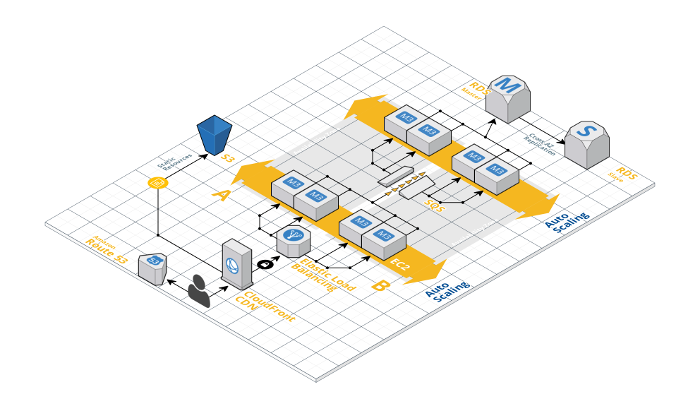
\includegraphics[width=0.8\textwidth]{figure/chapter-2-infrastructure-diagram.png}
    \caption{Contoh gambar}
    \label{fig:2.contoh}
\end{figure}

\subsubsection{Subsubbab} \label{II.Subsubbab1}

Berikut adalah contoh subsubbab. Ini adalah level subbab maksimal dalam laporan Tugas Akhir, dan tidak boleh lebih dalam.

\begin{figure}[H]
	\centering
	
\includegraphics[width=3cm]{figure/samplephoto.jpg}
	\caption{Contoh foto}
	\label{fig:2.foto}
\end{figure}

\subsection{Subbab 2} \label{II.Subbab2}
Untuk membuat sebuah persamaan, gunakan kode \verb|\begin{equation}| dibawah: \par

\begin{equation}
	x + 1 = 2
\end{equation}
\label{eq:2.sum}
\myequations{Fungsi x}

Berikut adalah contoh penulisan persamaan yang lebih kompleks, yaitu persamaan distribusi normal. \par

\begin{equation}
	P(x) = \frac{1}{{\sigma \sqrt {2\pi } }}e^{{{ - \left( {x - \mu } \right)^2 } \mathord{\left/ {\vphantom {{ - \left( {x - \mu } \right)^2 } {2\sigma ^2 }}} \right. \kern-\nulldelimiterspace} {2\sigma ^2 }}}
\end{equation}
\label{eq:2.normal}
\myequations{Distribusi normal}

Jika menuliskan banyak persamaan secara berurutan, gunakan  \verb|\begin{align}| atau \verb|\begin{gather}|: \par

\begin{align} 
	2x - 5y &=  8 \\ 
	3x + 9y &=  -12
\end{align}
\label{eq:2.SPL}
\myequations{Sistem persamaan linier}

    \newpage
\chapter{Analisis dan Perancangan} \label{Bab III}

\section{Alur Penelitian} \label{III.Alur}
Digambarkan terkait bagaimana proses yang dilakukan dalam penelitian, dari awal sampai dengan akhir. Gambarkan dalam bentuk diagram alir (\textit{flowchart}). \par

\section{Penjabaran Langkah Penelitian} \label{III.Jabar Alur}
Penjelasan detail dari langkah-langkah alur penelitian, yang sudah tergambar dalam flowchart di subbab \ref{III.Alur}. Subsubbab berikut harus sesuai dengan jumlah alur penelitian. \par

\subsection{Langkah 1} \label{III.Langkah 1}
Penjelasan Langkah 1. \par

\subsection{Langkah 2} \label{III.Langkah 2}
Penjelasan Langkah 2. \par

\section{Alat dan Bahan Tugas Akhir} \label{III.Alat dan Bahan}
Berisi alat-alat dan bahan-bahan yang digunakan dalam penelitian. \par

\subsection{Alat} \label{III.Alat}
Alat yang digunakan untuk melakukan penelitian, dapat berupa computer, PC, Arduino, raspberry, etc. Contoh: \par
\begin{enumerate}[noitemsep]
	\item \textit{Notebook} dengan spesifikasi minumum sistem operasi Windows 11, processor AMD Ryzen 5 7430 CPU @ 6 core/2,3 GHz, RAM 16GB DDR4, grafis AMD Radeon RX Vega 7 2GB, SSD 512 GB.
	\item \textit{Smartphone} dengan spesifikasi OS Android OS 12, CPU Snapdragon 778G Octa-core, GPU Adreno 642L, memori 128 GB, RAM 6 GB.
	\item Platform game engine Godot v4.3
	\item Code editor Microsoft Visual Studio Code
	\item Github
\end{enumerate}

\subsection{Bahan} \label{III.Bahan}
Bahan yang digunakan/diperlukan untuk melakukan penelitian, dapat berupa: \par
\begin{enumerate}[noitemsep]
	\item Dataset pihak lain yang diperoleh dengan izin atau dalam lisensi yang diizinkan untuk digunakan secara langsung,
	\item Dataset pihak pertama yang disusun sendiri melalui quisioner, observasi, atau interview,
	\item Dokumen panduan yang mengacu pada standar, hasil tugas akhir, atau artikel yang disitasi dan digunakan. 
\end{enumerate}

\section{Metode Pengembangan/Pengukuran} \label{III.Metode}
Membahas mengenai metode yang digunakan dalam penelitian, berdasarkan dasar teori yang sebelumnya sudah dijelaskan pada subbab \ref{II.Teori}. Setiap Tugas Akhir wajib memiliki metode dalam pelaksanaannya yang sesuai dengan penelitian yang dikerjakan: \par
\begin{enumerate}[noitemsep]
	\item Alur pengembangan tugas akhir, menggunakan flowchart
	\item Cara pengumpulan data yang digunakan ()Kuesioner, Wawancara, pengujian, dan lainnya)
	\item Metode pengembangan tugas akhir (Metode Waterfall, Agile, RAD, dan lainnya).
\end{enumerate}
Subbab ini akan berhubungan erat dengan Subbab \ref{IV.Hasil}. \par

\section{Ilustrasi Metode Pengembangan/Pengukuran} \label{III.Ilustrasi}
Jelaskan contoh perhitungan dari metode pengemubangan bagi penelitian Tugas Akhir yang menggunakan algoritma perhitungan tertentu. Tidak perlu harus menggunakan seluruh dataset, cukup menggunakan sampel data. Tujuannya untuk menggambarkan alur perhitungan metode dari data awal sampai luaran yang ditargetkan. \par

\section{Rancangan Pengujian} \label{III.Rancang Uji}
Penjabaran terkait rancangan \& skenario pengujian pada penelitian. Dapat berupa pengujian perangkat keras, lunak, fungsional, dan non-fungsional. Subbab ini akan berhubungan erat dengan Subbab \ref{IV.Uji}. \par
    \newpage
\chapter{Hasil dan Pembahasan} \label{Bab IV}

\section{Hasil Penelitian} \label{IV.Hasil}
Berisi hasil penelitian berdasarkan rancangan yang sudah dijelaskan pada Bab \ref{Bab III}, terutama dari Subbab \ref{III.Metode}. Bagi yang membuat alat, jelaskan alat yang jadi dalam bentuk apa. Bagi yang membuat aplikasi, jelaskan aplikasi yang jadi dalam bentuk seperti apa. Jabarkan dalam bentuk pseudocode dan dijelaskan per bagian kodenya. Gunakan gambar dan tabel sebagai alat bantu menjelaskan hasil. \par

\section{Hasil Pengujian} \label{IV.Uji}
Berikan hasil pengujian berdasarkan rancangan \& skenario yang sudah direncanakan sebelumnya pada Subbab \ref{III.Rancang Uji}. \par

\begin{longtable}{|c|c|c|}
	\caption{Contoh Hasil Pengujian}
	\label{table:4.uji}\\
	\hline
	\textbf{Pengujian} & \textbf{Metode A} & \textbf{Metode B} \\
	\hline
	\endhead
	Kecepatan & 10 ms & 12 ms \\ 
	\hline
	Memori & 10 MB & 7 MB \\
	\hline
\end{longtable}

\begin{figure}[H]
	\centering
	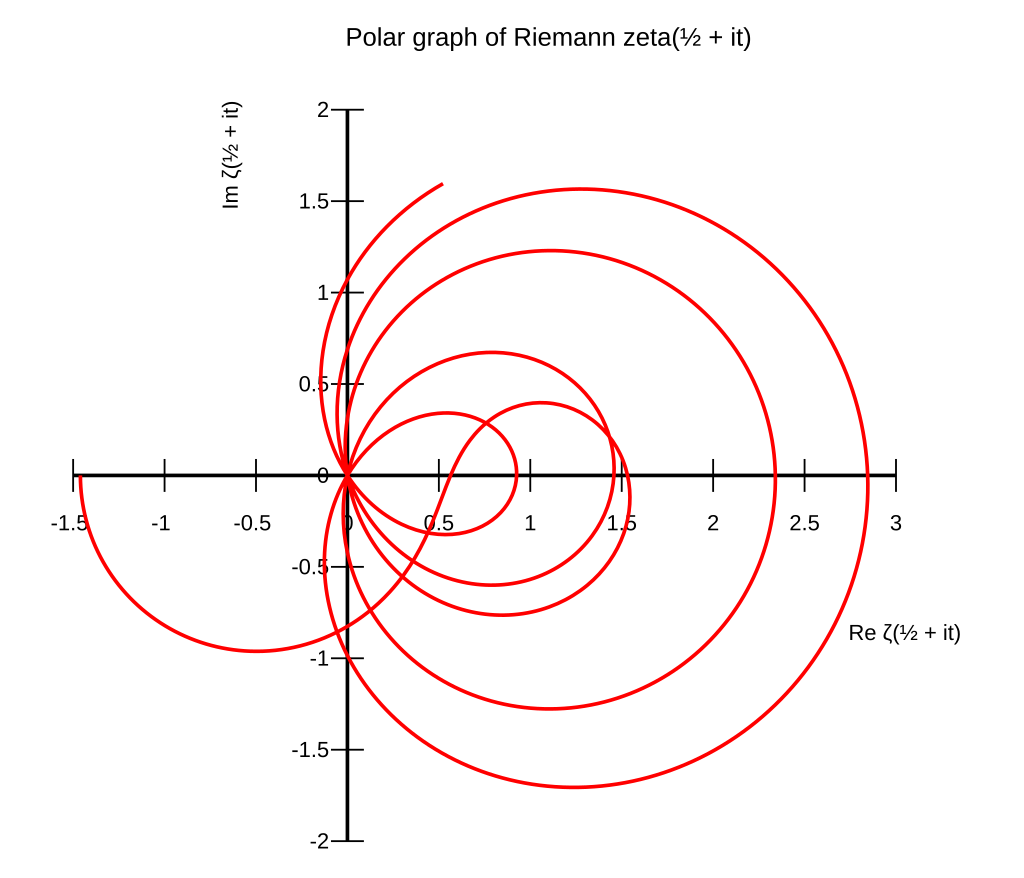
\includegraphics[width=0.5\textwidth]{figure/zeta.png}
	\caption{Contoh Graf Pengujian}
	\label{fig:4.graf}
\end{figure}

\section{Analisis Hasil Penelitian} \label{IV.Analisis}
Berikan analisis hasil penelitian \& pengujian, berupa data yang didapatkan dari penelitian \& pengujian Tugas Akhir yang sudah anda kerjakan. Gunakan gambar dan tabel sebagai alat bantu menjelaskan analisis hasil. Data luaran penelitian yang dapat dianalisis berupa: \par
\begin{enumerate}[noitemsep]
	\item Hasil pengujian
	\item Hasil kuesioner
	\item Aplikasi yang dikembangkan
\end{enumerate}
Analisis dapat membandingkan dengan hasil penelitian sebelumnya yang memiliki kemiripan topik. \par

\section{Pembahasan} \label{IV.Bahas}
Berisi pembahasan terkait hasil yang sudah didapatkan/dipaparkan sebelumnya, berupa penutup yang dapat menjelaskan mengenai kelebihan hasil tugas akhir dan kekurangannya dibandingkan dengan penelitian atau produk lain yang serupa atau mirip. \par
    \newpage
\chapter{KESIMPULAN DAN SARAN} \label{Bab V}

\section{Kesimpulan} \label{V.Kesimpulan}
Berdasarkan penelitian yang telah dilakukan, maka kesimpulan yang diperoleh adalah sebagai berikut:
\begin{enumerate}
    \item Berdasarkan pengujian 
    \item mengimplementasikan
\end{enumerate}

\section{Saran} \label{V.Saran}
Adapun saran yang dapat diberikan untuk penelitian lebih lanjut berdasarkan penelitian ini adalah sebagai berikut:\par
\begin{enumerate}
    \item Pengembangan 
    \item Tampilan 
\end{enumerate}
    %----------------------------------------------------------------%

    % Daftar Pustaka
    \newpage
    \phantomsection% 
    \addcontentsline{toc}{chapter}{DAFTAR PUSTAKA}
    \printbibliography[title={Daftar Pustaka}]

    % Lampiran
    % TODO: Tabel Lampiran
    \newpage
    \appendix
    \addcontentsline{toc}{chapter}{LAMPIRAN}
    \chapter*{Lampiran}
    \renewcommand\thesection{\Alph{section}}
    \section{Dataset}

\section{Hasil Wawancara}

\section{Rincian Kasus Uji}


\end{document}
